% =============================================================================
% VERITAS-Bench -- Springer LNCS / CCIS format (12 pages), matching the
% structure of the user-supplied reference (llncs, TikZ diagrams, tables).
%
% TARGET: Springer CCIS/LNCS venues (icSoftComp 2026, ICACDS 2026, CVIP 2026,
%         ICCIDS 2027). NOT IEEE (IEEE uses the 6-page IEEEtran version).
%
% HOW TO COMPILE (Overleaf): New Project -> upload this file + the figures/
% folder. It is self-contained (manual thebibliography, TikZ diagrams), so it
% compiles with the stock llncs class Overleaf provides. Compiler: pdfLaTeX.
%
% BEFORE SUBMITTING:
%   * Confirm the author list / affiliation / emails in the \author + \institute
%     blocks below.
%   * Keep <= 12 pages (Springer CCIS single-column limit; verify per venue).
%   * Every numeric value here is verified against a committed results/*.json.
% =============================================================================
\documentclass[runningheads]{llncs}
\usepackage{graphicx}
\usepackage{booktabs}
\usepackage{multirow}
\usepackage{amsmath}
\usepackage{amssymb}
\usepackage{hyperref}
\usepackage{tikz}
\usetikzlibrary{arrows.meta, positioning, shapes.geometric, fit, backgrounds}
\graphicspath{{figures/}}
\newcommand{\ns}{\textit{n.s.}}

\begin{document}

\title{VERITAS-Bench: A Validity Test-Suite and Confound Audit for Training-Free
Self-Supervised Dysarthric-Speech Severity Metrics}

% ---------------------------------------------------------------------------
% TODO (confirm): author list, affiliation, emails.
% Reference file lists two authors; VERITAS was described throughout as a solo
% project, so the primary author is shown here. Add a co-author if appropriate.
% ---------------------------------------------------------------------------
\author{Shaurya Punj}
\institute{Thapar Institute of Engineering and Technology, Patiala, Punjab, India \\
\email{shauryapunj@thapar.edu}}

\maketitle

\begin{abstract}
Training-free clinical-speech metrics built on frozen self-supervised (SSL)
speech models are proliferating: a dysarthria-severity score is obtained by
comparing a patient's frozen embeddings against healthy-control references, with
no labels and no fine-tuning. Such a metric is almost always validated by a
single number---a correlation with clinical severity on one corpus. We argue
that this is not validation, and we supply the missing procedure. We first audit
four popular metric families on real dysarthric speech (TORGO, $n{=}15$ graded,
with AG500 electromagnetic articulography; IPVS, $n{=}61$; EasyCall, $n{=}55$)
and show that every metric that ``passes'' a headline correlation
($\rho{=}0.74$--$0.77$) fails at least one validity control: its signal is
largely carried by silence (speech-only retention as low as $24\%$), its
representation is almost perfectly speaker-identifiable (AUC $0.996$--$0.999$),
or it does not transfer across corpora. A GT-free cycle-consistency reliability
metric carries no information about \emph{real} articulatory-inversion error once
speech energy is partialled out (partial Spearman $=-0.001$ over $22{,}854$ EMA
frames), and inversion-derived kinematics are artifacts. We then package the
controls that expose these confounds as \textbf{VERITAS-Bench}, a released
validity test-suite that runs six confound controls on \emph{any} per-speaker
metric and emits a machine-readable PASS/WARN/FAIL report card. Auditing an
independent reimplementation of the strongest published training-free metric
family, the suite certifies it as silence-, energy- and leakage-robust while
surfacing a confound no published metric reports checking. VERITAS-Bench turns
metric validity from an assumption into a checkable artifact.
\end{abstract}

\keywords{Dysarthria \and Self-supervised speech models \and Clinical speech
assessment \and Benchmark \and Validity \and Confounds \and
Articulatory inversion}

% ===========================================================================
\section{Introduction}
% ===========================================================================
Dysarthria is a motor-speech disorder in which impaired control of the
articulators degrades intelligibility; it accompanies conditions such as
Parkinson's disease, amyotrophic lateral sclerosis (ALS), cerebral palsy and
stroke. Objective, automatic severity assessment promises consistent monitoring
and scalable screening, but supervised approaches are limited by the scarcity of
labelled pathological speech. This scarcity has motivated a wave of
\textbf{training-free} metrics built on \emph{frozen} self-supervised (SSL)
speech models such as WavLM~\cite{chen2022wavlm} and
HuBERT~\cite{hsu2021hubert}, whose representations encode rich phonetic and
articulatory structure without any task-specific training~\cite{mohamed2022review}.
A typical training-free metric compares a patient's frozen embeddings to a
healthy-control reference and reports the distance as a severity score.

The evidence offered for such a metric is almost always the same: a single
Spearman correlation with clinical severity, measured on one corpus. That number
is necessary but far from sufficient. A metric can correlate with severity
because it measures the disorder---or because it measures how long the speaker
pauses, how loudly they speak, or simply \emph{who they are}. These are not
hypothetical confounds; we show that all three occur in metrics currently in
use. What the field lacks is not another metric, but a \textbf{standard procedure
for deciding whether a metric measures what it claims}.

This paper contributes that procedure. We first conduct a systematic audit that
establishes, on real dysarthric speech and against real articulatory ground
truth, that four popular metric families are confounded. We then distil the
controls that expose those confounds into \textbf{VERITAS-Bench}, a released,
metric-agnostic validity test-suite that audits any per-speaker clinical-speech
metric against six controls and returns a PASS/WARN/FAIL report card. Finally, we
use the suite to audit an independent reimplementation of the strongest published
training-free metric family, demonstrating that the tool discriminates---
certifying good design where it is present rather than merely failing everything.

The primary contributions of this paper are:
\begin{itemize}
\item A systematic validity audit of four training-free frozen-SSL severity
metric families on three real corpora ($n{=}131$ speakers, two languages),
grounded against real electromagnetic articulography (EMA).
\item Five reproducible confound findings---speaker-identity leakage, silence
dependence, energy artifacts, cross-corpus fragility, and inversion
instability---each with a concrete, reusable diagnostic.
\item A leave-one-control-out (LOCO) reference-construction protocol that removes
speaker-identity leakage from reference-based metrics and quantifies the inflation
it eliminates.
\item \textbf{VERITAS-Bench}, a released validity test-suite with a documented
threshold policy, a metric-agnostic plug-in interface, and a machine-readable
report-card schema.
\item An audit of an independent reimplementation of the strongest published
training-free metric family, showing the suite both validates sound design and
surfaces a previously unreported confound.
\item A reproducible release---code, thresholds, and all report cards---so that
any claimed clinical-speech metric can be audited by its authors, reviewers, or
users.
\end{itemize}

% ===========================================================================
\section{Related Work}
% ===========================================================================
Prior work relevant to this study spans self-supervised speech representations,
training-free clinical metrics, the known confounds of pathological-speech
modelling, and the practice of benchmarking. We organise it below.

\textbf{Self-Supervised Speech Representations:} Models such as
wav2vec~2.0~\cite{baevski2020wav2vec2}, HuBERT~\cite{hsu2021hubert} and
WavLM~\cite{chen2022wavlm} learn general-purpose speech representations from
unlabelled audio and have become the default feature extractor for downstream
tasks~\cite{mohamed2022review}. These transformer-based
models~\cite{vaswani2017attention}, following the masked-pretraining paradigm
popularised for text~\cite{devlin2019bert} and scaled for speech under weak
supervision~\cite{radford2023whisper}, are typically pre-trained on read English
speech such as LibriSpeech~\cite{panayotov2015librispeech}---a domain mismatch
that itself matters for pathological speech. Probing studies such as
SUPERB~\cite{yang2021superb}
show that different layers encode different information---lower layers speaker and
acoustic detail, middle layers phonetic content---a layer-wise structure that is
central to the confounds we study.

\textbf{Training-Free Clinical-Speech Metrics:} Because labelled dysarthric speech
is scarce, a growing literature derives severity scores directly from frozen SSL
features without fine-tuning. Approaches include pooled-embedding regression,
reference-distance scores that compare a patient's trajectory to healthy
controls, and articulatory-inversion analyses. The strongest current example
estimates phonological-feature directions from healthy-control speech in a frozen
model and scores a speaker by the $d'$ separation of their phone embeddings along
those directions, reporting severity correlations across thousands of speakers,
many languages and several aetiologies~\cite{muller2026cross,muller2026collapse};
such methods are typically evaluated on dysarthria corpora such as
UA-Speech~\cite{kim2008uaspeech}. That work carefully controls token count and
alignment quality; we show it is also
silence-, energy- and leakage-robust, while noting the one confound it does not
report checking.

\textbf{Speaker Information in SSL Representations:} Early SSL layers encode
speaker identity strongly, a property exploited by speaker-verification and
health-diagnostic models but a liability for reference-based clinical metrics: a
score that partly reflects \emph{who} the speaker is will correlate with any
speaker-correlated label~\cite{zhu2024wavrx}. We operationalise this both as a
reference-construction confound and as a representation-level identifiability
probe.

\textbf{Confounds in Pathological-Speech Modelling:} Silence and pausing, recording
energy, and corpus-specific idiosyncrasy are long-suspected confounds in clinical
speech, but are rarely controlled jointly or reported as validity checks. Forced
alignment~\cite{mcauliffe2017mfa} enables a principled silence/speech split, which
we use to quantify how much of a metric's signal survives silence removal.

\textbf{Acoustic-to-Articulatory Inversion:} Frozen SSL features can be inverted
to articulatory trajectories; SPARC~\cite{cho2024sparc} maps audio to vocal-tract
kinematics and back. We test whether inversion-derived reliability and kinematic
signals hold up against \emph{measured} articulation (EMA), which most inversion
work cannot access.

\textbf{Benchmarking and Validity:} Existing clinical-speech benchmarks rank
\emph{systems by accuracy}. To our knowledge, none audit \emph{whether a metric's
accuracy is confounded}. VERITAS-Bench is a validity benchmark rather than a
leaderboard: a metric does not win by scoring highest, but by surviving the
controls.

% ===========================================================================
\section{System Architecture}
% ===========================================================================
VERITAS-Bench is organised as a layered pipeline (Fig.~\ref{fig:arch}) that turns
any per-speaker metric and any corpus into a machine-readable validity report
card. The design goal is that auditing a new metric costs a few lines of code and
no change to the battery.

\textbf{Corpus Adapter Layer:} Each corpus is exposed through a loader that yields
per-speaker \emph{views}. A view carries the speaker's pooled frozen-SSL features
(full and silence-trimmed), a mean speech-energy value, the graded or binary
severity label, and a control/patient flag. New corpora are added by implementing
one loader; the battery is unchanged.

\textbf{Metric Interface:} A metric implements a single required method,
\texttt{predictive\_scores(views)}, returning $\{\text{speaker}\rightarrow
\text{score}\}$ with the convention that \emph{higher $=$ more severe}. Two
optional overrides unlock further controls: \texttt{loco\_scores} enables the
leakage test for reference-based metrics, and a \texttt{has\_representation} flag
exposes the metric's underlying features to the transfer and identity probes.

\textbf{The Six-Control Battery:} The core of the system runs six independent
validity controls (Section~\ref{sec:controls}) over the metric and corpus,
verifying speaker-disjointness at every step and failing loudly on contract
violations.

\textbf{Threshold Policy:} Every PASS/WARN/FAIL boundary is a single, documented
policy constant, collected in one place so that a report card is auditable and a
reviewer can re-interpret it under a different policy without re-running anything.

\textbf{Report-Card Layer:} Outcomes are serialised to a plain JSON report card
(one per metric $\times$ corpus): for each control an outcome, a one-line headline
carrying the load-bearing number, and the raw statistics, plus the threshold
policy that produced the verdicts. Cards are diff-able in version control, so a
metric's validity can be tracked as it evolves.

\textbf{Reproducibility Layer:} All randomness is seeded; frozen model weights are
loaded from a local cache; splits are speaker-disjoint throughout; and every
headline number in a card maps to a committed result file. The suite is
self-demonstrating: run on the paper's own metrics, it reproduces the paper's
findings exactly.

\begin{figure}[t]
\centering
\resizebox{\textwidth}{!}{%
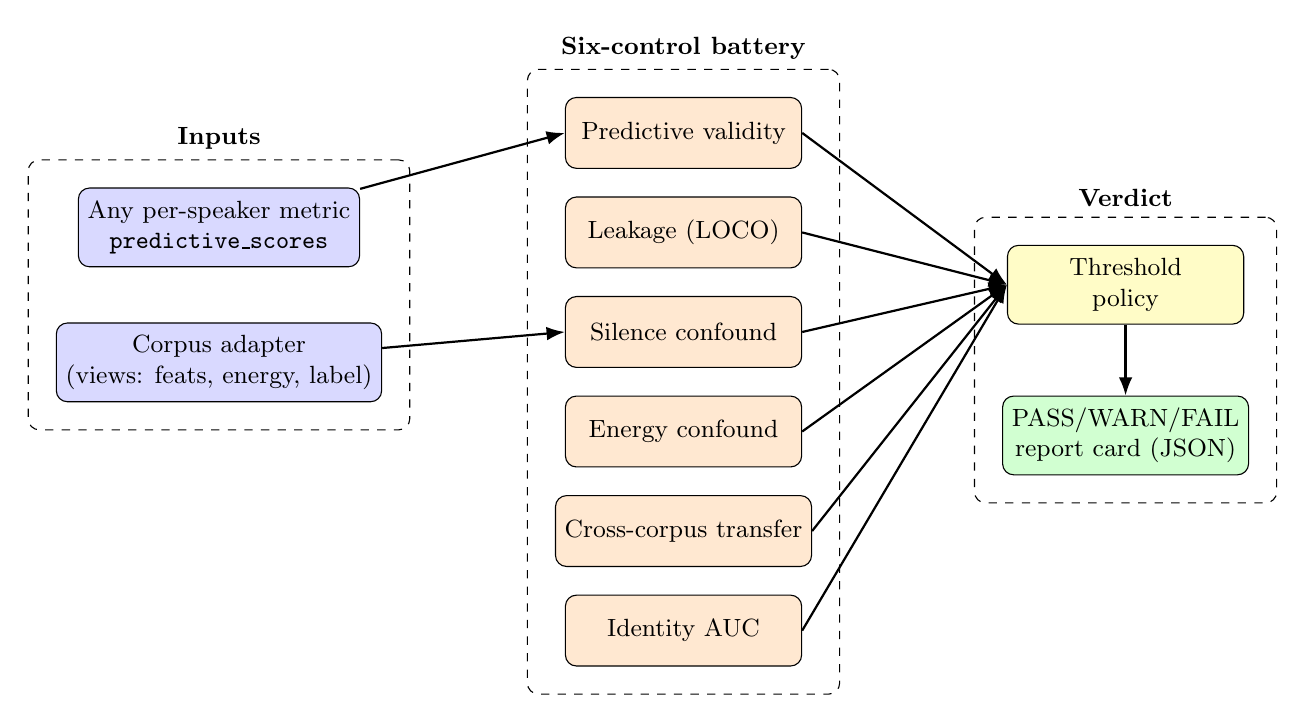
\begin{tikzpicture}[
    font=\small,
    arrow/.style={-{Latex}, thick},
    box/.style={rectangle, rounded corners, draw, align=center, minimum height=1cm, minimum width=3.0cm},
    ctrl/.style={rectangle, rounded corners, draw, align=center, minimum height=0.9cm, minimum width=3.0cm, fill=orange!18},
    group/.style={rectangle, draw, dashed, rounded corners, inner sep=0.35cm}
]
% inputs
\node[box, fill=blue!15] (metric) {Any per-speaker metric\\\texttt{predictive\_scores}};
\node[box, fill=blue!15, below=0.7cm of metric] (corpus) {Corpus adapter\\(views: feats, energy, label)};
% controls column
\node[ctrl, right=2.6cm of metric, yshift=1.2cm] (c1) {Predictive validity};
\node[ctrl, below=0.35cm of c1] (c2) {Leakage (LOCO)};
\node[ctrl, below=0.35cm of c2] (c3) {Silence confound};
\node[ctrl, below=0.35cm of c3] (c4) {Energy confound};
\node[ctrl, below=0.35cm of c4] (c5) {Cross-corpus transfer};
\node[ctrl, below=0.35cm of c5] (c6) {Identity AUC};
% thresholds + card
\node[box, fill=yellow!22, right=2.6cm of c3, yshift=0.6cm] (thr) {Threshold\\policy};
\node[box, fill=green!18, below=0.9cm of thr] (card) {PASS/WARN/FAIL\\report card (JSON)};
% arrows
\draw[arrow] (metric) -- (c1.west);
\draw[arrow] (corpus) -- (c3.west);
\foreach \c in {c1,c2,c3,c4,c5,c6}{\draw[arrow] (\c.east) -- (thr.west);}
\draw[arrow] (thr) -- (card);
% groups
\node[group, fit=(metric)(corpus), label=above:{\textbf{Inputs}}] {};
\node[group, fit=(c1)(c2)(c3)(c4)(c5)(c6), label=above:{\textbf{Six-control battery}}] {};
\node[group, fit=(thr)(card), label=above:{\textbf{Verdict}}] {};
\end{tikzpicture}
}
\caption{VERITAS-Bench architecture. Any per-speaker metric and any corpus adapter
feed a six-control validity battery whose outcomes are combined under a documented
threshold policy into a machine-readable PASS/WARN/FAIL report card.}
\label{fig:arch}
\end{figure}

% ===========================================================================
\section{The Six Validity Controls}
\label{sec:controls}
% ===========================================================================
Every threshold below is a stated policy choice, documented in one place so a card
is auditable. Significance uses $\alpha{=}0.05$ throughout; the overall verdict is
the \emph{worst applicable} control (not-applicable controls are ignored unless all
are).

\textbf{Predictive Validity:} the within-corpus, leave-one-speaker-out Spearman
$\rho$ between the metric and clinical severity. A metric that cannot recover
severity within a single speaker-disjoint corpus is not measuring the disorder at
all. PASS requires $\rho{\ge}0.50$ and $p{<}\alpha$; WARN $\rho{\ge}0.30$; else
FAIL.

\textbf{Speaker-Identity Leakage (LOCO):} for reference-based metrics,
$\Delta = \rho(\text{naive reference}) - \rho(\text{leave-one-control-out
reference})$. A reference (or a fitted direction) that contains the test speaker's
own control data inflates that speaker's score. The LOCO protocol
(Fig.~\ref{fig:loco}) rebuilds the reference excluding the test speaker; $\Delta$
is the correlation that was pure leakage. PASS $\Delta{\le}0.05$; WARN
$\Delta{\le}0.15$; else FAIL.

\textbf{Silence Confound:} using forced alignment~\cite{mcauliffe2017mfa} we split
frames into silence and speech, and compute retention
$=\rho(\text{speech-only})/\rho(\text{full})$ together with the mean silence-frame
fraction. A metric whose signal lives in the silences is measuring pausing, not
articulation. PASS if retention $\ge0.70$ \emph{and} silence fraction $<0.50$;
WARN if retention $\ge0.40$ or the representation is majority silence; else FAIL.

\textbf{Energy Confound:} the partial Spearman between the metric and severity
controlling for mean speech log-RMS energy, relative to the raw correlation. If
loudness explains the correlation, the metric is an energy artifact. PASS if the
partial retains $\ge70\%$ of the raw $\rho$; WARN $\ge40\%$; else FAIL.

\textbf{Cross-Corpus Transfer:} the metric's representation is used to train a
severity probe on the other corpora and test on the held-out corpus. Single-corpus
success that does not transfer is overfitting to corpus idiosyncrasy. PASS
$\rho{\ge}0.50$ and $p{<}\alpha$; WARN $\rho{\ge}0.30$ and $p{<}\alpha$; else FAIL.

\textbf{Representation Identifiability:} the macro one-vs-rest
speaker-classification AUC of the representation the metric uses (chance $0.5$).
High identifiability is a leakage \emph{risk} for any reference-based metric built
on the features. PASS AUC $\le0.70$; WARN $\le0.85$; else FAIL.

\begin{figure}[t]
\centering
\resizebox{0.92\textwidth}{!}{%
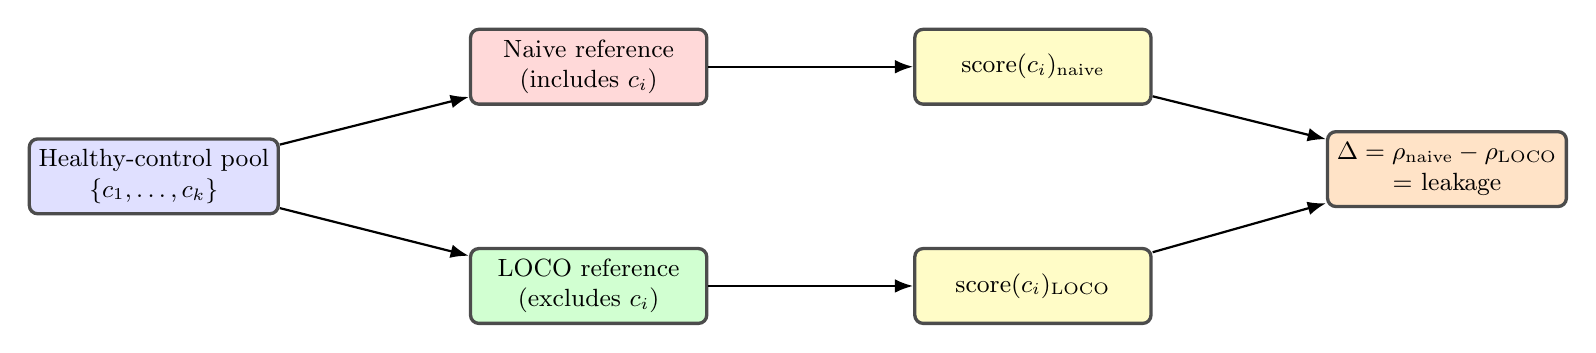
\begin{tikzpicture}[
    font=\small, node distance=1.9cm, >={Latex},
    st/.style={rectangle, rounded corners=3pt, draw=black!70, very thick, align=center, minimum width=3.0cm, minimum height=0.95cm},
    naive/.style={st, fill=red!15}, loco/.style={st, fill=green!18}, sc/.style={st, fill=blue!12},
    arrow/.style={->, thick}
]
\node[sc] (pool) {Healthy-control pool\\$\{c_1,\dots,c_k\}$};
\node[naive, above right=0.4cm and 2.4cm of pool] (naiveref) {Naive reference\\(includes $c_i$)};
\node[loco, below right=0.4cm and 2.4cm of pool] (locoref) {LOCO reference\\(excludes $c_i$)};
\node[st, fill=yellow!22, right=2.6cm of naiveref] (sn) {score($c_i$)$_\text{naive}$};
\node[st, fill=yellow!22, right=2.6cm of locoref] (sl) {score($c_i$)$_\text{LOCO}$};
\node[st, fill=orange!22, right=2.2cm of sn, yshift=-1.3cm] (delta) {$\Delta=\rho_\text{naive}-\rho_\text{LOCO}$\\= leakage};
\draw[arrow] (pool) -- (naiveref);
\draw[arrow] (pool) -- (locoref);
\draw[arrow] (naiveref) -- (sn);
\draw[arrow] (locoref) -- (sl);
\draw[arrow] (sn) -- (delta);
\draw[arrow] (sl) -- (delta);
\end{tikzpicture}
}
\caption{The leave-one-control-out (LOCO) protocol. Scoring a control speaker
$c_i$ against a reference that contains $c_i$'s own data leaks speaker identity;
rebuilding the reference without $c_i$ isolates the inflation $\Delta$.}
\label{fig:loco}
\end{figure}

% ===========================================================================
\section{Metrics Under Audit}
% ===========================================================================
We audit four metrics, chosen to span the popular training-free families and to
include the current state of the art. All are computed on the same frozen
WavLM-Large features and the same alignments, so the comparison is like-for-like.

\textbf{ATD (Articulatory Trajectory Deviation):} a reference-distance metric.
Each speaker's frozen-WavLM trajectory (reduced to 64 principal components) is
compared to a per-word healthy-control reference by length-normalised dynamic time
warping; the speaker-mean distance is the severity score. We evaluate it at a
mid-network layer (\textbf{ATD-L9}) and an early layer (\textbf{ATD-L1}).

\textbf{Pooled-Embedding Probe:} a probe-kind metric. Frozen WavLM-L9 features are
mean-pooled per utterance and per speaker; a regularised linear regressor
(Ridge/LinearSVR, nested cross-validation) predicts severity. This is the fair,
tuned baseline that reference-geometry methods must beat.

\textbf{Phonological-Subspace $d'$:} an independent reimplementation---\emph{from
the published description, not the authors' code}---of the strongest current
training-free family~\cite{muller2026cross,muller2026collapse}. Phone-level
embeddings are extracted via forced alignment; a direction for each binary
phonological contrast (nasality, voicing, stridency, sonorance, continuancy) is
estimated \emph{from healthy controls only}; each speaker is scored by the $d'$
separation of their phone embeddings along those directions, with score
$=-\overline{d'}$ (degraded contrasts $\Rightarrow$ lower $d'\Rightarrow$ more
severe). Because the directions are fitted on the control pool, this is naturally a
\emph{reference} metric, and the leakage control applies.

% ===========================================================================
\section{Data and Experimental Setup}
% ===========================================================================
\textbf{Corpora.} \textbf{TORGO}~\cite{rudzicz2012torgo} provides 15 English
speakers (8 dysarthric, cerebral-palsy/ALS; 7 control) with audio, AG500 3-D
electromagnetic articulography at 200\,Hz, and graded severity $\{0,1,2\}$; it is
the only corpus here with graded severity \emph{and} measured articulation.
\textbf{IPVS}~\cite{dimauro2017ipvs} provides 61 Parkinsonian/control speakers and
\textbf{EasyCall}~\cite{turrisi2021easycall} 55 Italian speakers (31 dysarthric,
24 control); both public packages carry binary labels and serve as detection and
cross-corpus references.

\textbf{Articulatory ground truth.} Of the 7 dysarthric TORGO speakers with EMA
sessions, only 2 are usable ($\le 2$ dead sensor coils), and both are mild; every
severe dysarthric EMA session is degenerate (3--8 dead coils). This
$n{\approx}2$ ceiling is itself a finding: public \emph{dysarthric} articulatory
ground truth barely exists.

\textbf{Features and protocol.} All metrics use frozen
WavLM-Large~\cite{chen2022wavlm}; features are mean-pooled per utterance then per
speaker. Random seed 42; frozen weights; speaker-disjoint splits throughout. The
cross-corpus probe uses per-corpus z-rank label harmonisation and an 80-utterance
per-speaker cap; all other tests use every available utterance.

% ===========================================================================
\section{Experimental Evaluation}
% ===========================================================================
We report three groups of results: the within- versus cross-corpus behaviour that
motivates the transfer control; the confound findings that motivate the remaining
controls; and the report cards that VERITAS-Bench produces, including the audit of
the state-of-the-art metric.

\subsection{Within-Corpus Success, Cross-Corpus Fragility}
A fairly-tuned probe on frozen WavLM-L9 recovers severity strongly \emph{within}
corpus (Table~\ref{tab:xc}, Fig.~\ref{fig:xc}), reaching $\rho{=}0.74$--$0.85$.
Leave-one-corpus-out transfer, however, is heterogeneous: four of six cells remain
significant---binary detection partially transfers (EasyCall $\rho{=}0.64$,
$p{=}1{\times}10^{-7}$)---but transfer to the only graded corpus, TORGO, is not
significant ($\rho{=}0.43$, $p{=}0.11$). At $n{=}15$ the critical value is
$\rho{\approx}0.52$, so this is an \emph{underpowered null, not a proven absence}.
The honest lesson is that transfer is \emph{metric- and power-dependent} and must
be demonstrated per metric, not assumed---a failure mode invisible to
single-corpus evaluation.

\begin{table}[t]
\centering
\caption{Within-corpus (leave-one-speaker-out) versus leave-one-corpus-out (LOCO,
train on the other two) severity Spearman $\rho$ on frozen WavLM-L9.
$^{\dagger}$~not significant ($p{=}0.11$).}
\label{tab:xc}
\begin{tabular}{lclcc}
\toprule
Corpus & $n$ & Label & Within $\rho$ & LOCO $\rho$ \\
\midrule
TORGO    & 15 & graded $\{0,1,2\}$ & 0.74 & 0.43$^{\dagger}$ \\
IPVS     & 61 & binary PD/HC       & 0.85 & 0.27 \\
EasyCall & 55 & binary dys/HC      & 0.84 & 0.64 \\
\bottomrule
\end{tabular}
\end{table}

\begin{figure}[t]
\centering
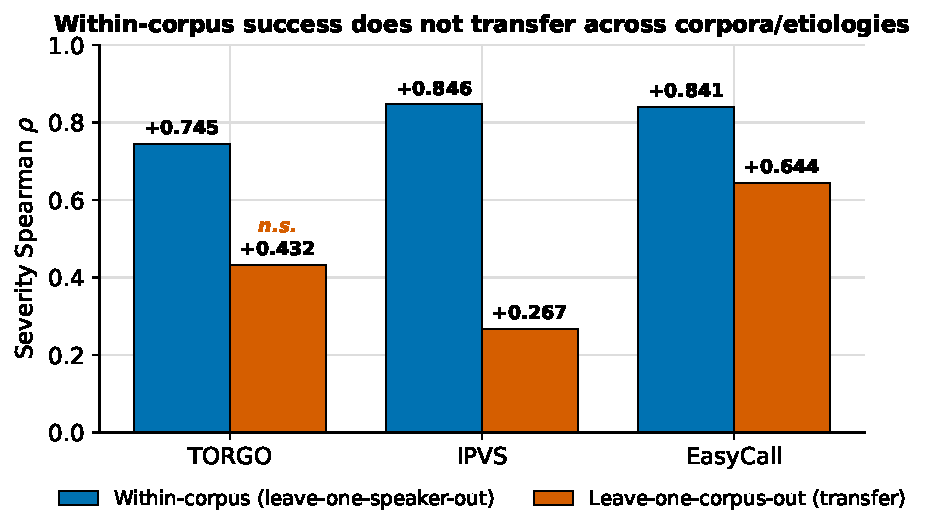
\includegraphics[width=0.72\textwidth]{fig1_within_vs_loco.pdf}
\caption{Within-corpus severity prediction is strong for all three corpora, but
leave-one-corpus-out transfer degrades and, for the only graded corpus (TORGO),
becomes non-significant.}
\label{fig:xc}
\end{figure}

\subsection{The Confound Findings}
\textbf{Speaker-identity leakage.} On TORGO a naive per-word reference gives an
early-layer (L1) score of $\rho{=}0.775$; under a strict LOCO reference it falls to
$0.687$ ($\Delta{=}0.089$). The mid-network layer (L9) is leakage-robust
($0.756{\to}0.756$). Early SSL layers encode speaker identity~\cite{zhu2024wavrx};
the LOCO protocol removes the inflation and shows that leakage is a hazard
specifically for early-layer reference metrics.

\textbf{Silence and pausing.} Decomposing the reference-distance signal by
alignment: the full metric tracks severity at $\rho{=}0.756$; silence frames
\emph{alone} reproduce it ($\rho{=}0.775$); silence-trimmed speech under a naive
reference collapses ($\rho{=}0.181$, \ns); but silence-trimmed speech under a LOCO
reference recovers ($\rho{=}0.644$, $p{=}0.010$). The raw metric therefore conflates
articulation, pausing and speaker identity, and only removing both isolates the
residual real signal.

\textbf{Cycle-consistency does not measure inversion reliability.} A natural
GT-free reliability metric inverts audio to articulation
(SPARC~\cite{cho2024sparc}), re-synthesises, and measures cycle-consistency. Tested
against \emph{real} EMA inversion error on TORGO controls ($n{=}5$ usable speakers,
$22{,}854$ frames, held-out affine alignment), the raw pooled Spearman is $+0.129$
but is a speech-energy artifact ($\rho_{\text{faith,energy}}{=}-0.468$); the
energy-controlled partial Spearman is $-0.001$. A healthy-manifold-centered variant
is $+0.39$---the wrong sign. Either way the metric carries no usable information
about real inversion error (Fig.~\ref{fig:cyc}).

\begin{figure}[t]
\centering
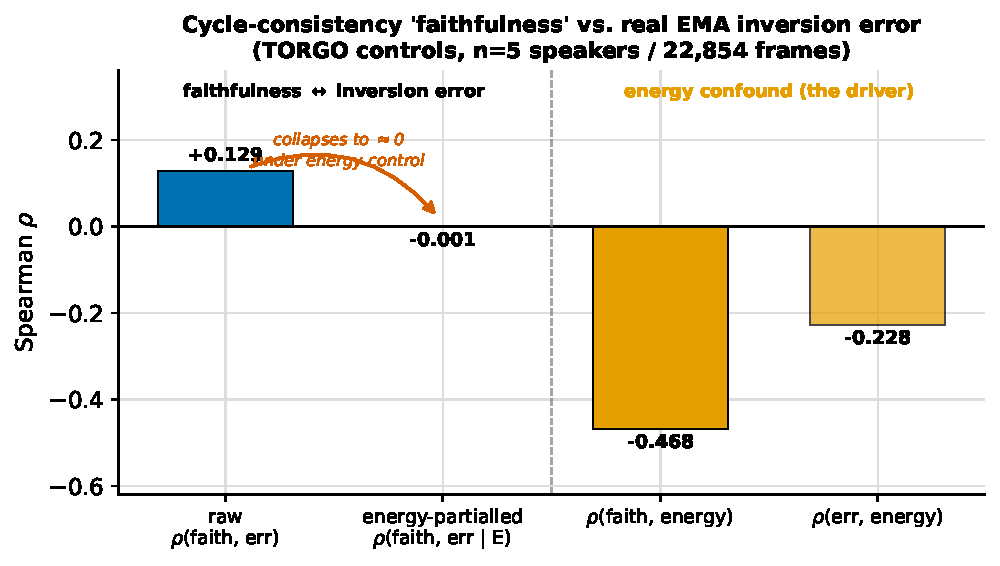
\includegraphics[width=0.70\textwidth]{fig3_cycle_consistency.pdf}
\caption{The raw faithfulness-versus-error association ($+0.129$) vanishes to
$-0.001$ once speech energy is partialled out, because both faithfulness and
inversion error are themselves driven by energy. Per-frame, TORGO controls,
$n{=}5$ / $22{,}854$ frames.}
\label{fig:cyc}
\end{figure}

\textbf{Inversion is unstable on disordered input.} Kinematic features (tongue
range, velocity) from SSL inversion do not track the measured EMA features
(grounding $\rho{=}0.39$, \ns); a ``significant'' range-versus-severity correlation
($\rho{=}+0.52$, $p{=}0.048$) is in the clinically wrong direction. Combined with the
$n{\approx}2$ dysarthric-EMA ceiling, this closes the door on validating pathological
inversion with public data.

\subsection{Report Cards and the State-of-the-Art Audit}
Table~\ref{tab:cards} is the central result: VERITAS-Bench applied to all four
metrics on TORGO. Every metric passes its headline predictive-validity correlation
($\rho{=}0.74$--$0.77$) and would, on the usual single-number evidence, be declared
successful. The card separates them.

\begin{table}[t]
\centering
\caption{VERITAS-Bench report cards on TORGO ($n{=}15$, real, seed 42). Every metric
passes predictive validity, yet each fails at least one confound control. The
phonological-subspace metric is our reimplementation of the state of the art.}
\label{tab:cards}
\begin{tabular}{lcccc}
\toprule
Control & ATD-L9 & ATD-L1 & Probe & Phono-sub. \\
\midrule
predictive validity      & PASS .77 & PASS .69 & PASS .74 & PASS .74 \\
leakage (LOCO $\Delta$)  & PASS .00 & WARN .09 & N/A      & PASS .00 \\
silence (kept)           & \textbf{FAIL} 24\% & --- & WARN 100\% & WARN 100\% \\
energy (kept)            & PASS 96\% & --- & PASS 80\% & PASS 88\% \\
cross-corpus             & \textbf{FAIL} \ns & --- & \textbf{FAIL} \ns & \textbf{FAIL} \ns \\
identity AUC             & \textbf{FAIL} .996 & --- & \textbf{FAIL} .996 & \textbf{FAIL} .999 \\
\midrule
\textbf{overall}         & \textbf{FAIL} & \textbf{WARN} & \textbf{FAIL} & \textbf{FAIL} \\
\bottomrule
\end{tabular}
\end{table}

\textbf{The battery discriminates.} The trajectory-distance metric loses $76\%$ of
its severity signal when silence is removed (retention $24\%$, FAIL): it substantially
measures pausing. The phonological-subspace metric retains $100\%$---it is
silence-free by construction, reading only frames inside aligned phones---and is
energy- and leakage-robust. A benchmark that returned FAIL for everything would be a
hit-piece; this one certifies a good design where the design is good.

\textbf{A confound the state of the art does not report checking.} Every
representation here is near-perfectly speaker-identifiable (AUC $0.996$--$0.999$).
Because this holds \emph{across all four metrics}, it is not a defect of any one of
them but a systemic property of the frozen SSL representation: any reference-based
clinical metric built on these features inherits a strong identity-leakage risk. The
phonological-subspace work reports controlling token count and alignment quality but
not identity leakage or energy; our audit supplies both, and the metric passes energy
and---because its per-contrast inflation is near-uniform across controls---leakage
ranking ($\Delta{=}0.000$), while inheriting the systemic identity risk.

\textbf{Cross-corpus, stated honestly.} All four metrics fail to transfer
significantly to the graded corpus ($\rho{=}0.43$--$0.47$, $p{\approx}0.08$--$0.11$),
but this is an underpowered null at $n{=}15$. The phonological-subspace work
demonstrates transfer at $n{\approx}3{,}374$; we do not claim otherwise. The battery
reports what the available graded data can support and labels the limit rather than
overclaiming.

\begin{table}[t]
\centering
\caption{Fair, tuned baselines on TORGO severity (leave-one-speaker-out, $n{=}15$).
A regularised pooled-embedding probe ties the zero-shot trajectory-distance score;
both beat an MFCC baseline.}
\label{tab:base}
\begin{tabular}{lc}
\toprule
Method & $\rho$ (LOSO) \\
\midrule
Reference-distance (zero-shot, frozen) & 0.756 \\
WavLM-L9 mean-pool $+$ Ridge            & 0.760 \\
WavLM-L9 mean-pool $+$ LinearSVR        & 0.775 \\
MFCC $+$ RBF-SVR                        & 0.609 \\
\bottomrule
\end{tabular}
\end{table}

\begin{figure}[t]
\centering
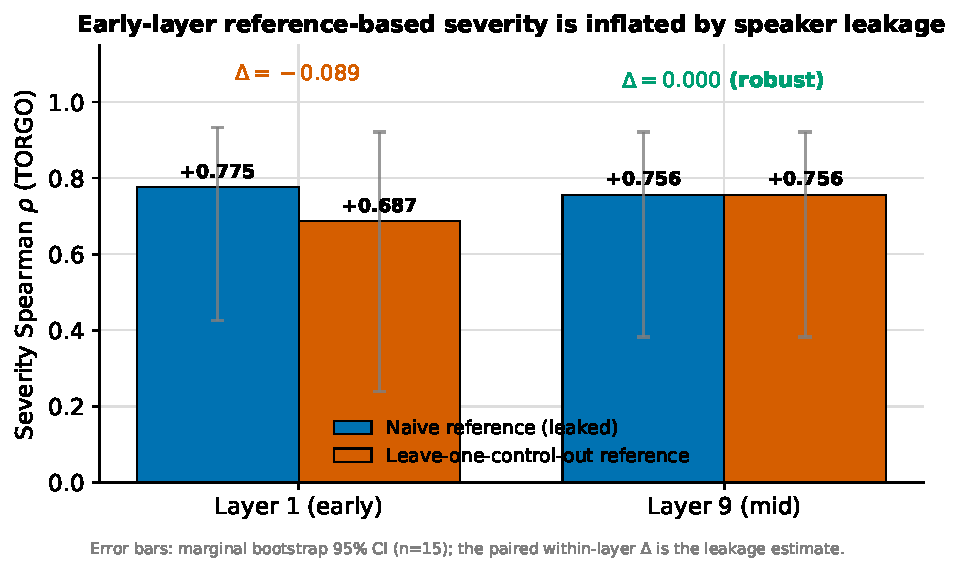
\includegraphics[width=0.72\textwidth]{fig2_leakage.pdf}
\caption{Reference-based severity on TORGO. The early layer (L1) drops
$\Delta{=}0.089$ from a naive to a leave-one-control-out reference---speaker
leakage---while the mid layer (L9) is unchanged.}
\label{fig:leak}
\end{figure}

\textbf{Key Findings.}
\begin{enumerate}
\item Every audited metric passes its headline correlation yet fails at least one
confound control; a single $\rho$ is not validation.
\item Speaker-identity leakage inflates early-layer reference metrics; the LOCO
protocol removes it and mid-network layers are robust.
\item The trajectory-distance signal is majority silence; the state-of-the-art
phonological-subspace metric is silence-robust by construction.
\item Cycle-consistency reliability and inversion kinematics do not survive validation
against measured articulation.
\item Near-perfect representation identifiability (AUC $0.996$--$0.999$) is a systemic
leakage risk for all reference metrics built on frozen SSL features.
\end{enumerate}

% ===========================================================================
\section{Discussion and Limitations}
% ===========================================================================
The report card is deliberately unflattering: no metric we tested, including the best
published one, passes every control. That is the intended function---a single headline
$\rho$ cannot distinguish a metric that measures articulation from one that measures
pausing, loudness or identity, and the community has lacked a standard way to tell them
apart. Six cheap controls do.

\textbf{Methodological Limitations:}
\begin{itemize}
\item \textbf{Sample size.} Graded severity is available for only $n{=}15$ speakers,
so the cross-corpus control is underpowered; its FAIL verdicts read as ``not
demonstrated,'' not ``disproved.''
\item \textbf{Reimplementation.} Our phonological-subspace metric follows the published
description, not the authors' code, so it is evidence about the \emph{design}, not a
replication of their exact numbers.
\item \textbf{Articulatory ground truth.} Usable dysarthric EMA is effectively
$n{\approx}2$, bounding any validation of pathological inversion.
\item \textbf{Thresholds.} PASS/WARN/FAIL boundaries are policy choices; they are stated
explicitly and changeable in one place, but they are choices.
\end{itemize}

\textbf{Threats to Validity:}
\begin{itemize}
\item Forced-alignment error can shift the silence/speech split; we mitigate by using a
standard aligner and reporting the silence fraction alongside retention.
\item The identity-AUC probe measures identifiability of the representation, which is a
\emph{risk} indicator; it need not manifest as rank inflation on every corpus, as the
near-uniform phonological-subspace leakage shows.
\end{itemize}

\textbf{Ethical Considerations:}
\begin{itemize}
\item A severity metric that partly encodes speaker identity risks systematic bias
across demographic groups; identity-leakage auditing is therefore a fairness concern,
not only a correctness one.
\item Clinical deployment of an unvalidated metric can mislead assessment; releasing an
audit tool is intended to raise the evidentiary bar before deployment.
\end{itemize}

\textbf{Generalisation:} the controls are corpus- and language-agnostic by construction;
the same metric can be audited on any corpus with a loader. The findings here are
English/Italian and small-$n$ for graded severity; broader graded corpora would
strengthen the transfer control specifically.

% ===========================================================================
\section{Conclusion and Future Work}
% ===========================================================================
Frozen-SSL clinical-speech metrics are easy to build, easy to validate badly, and easy
to fool. We audited four training-free severity metric families on real dysarthric speech
and against real articulatory ground truth, showed that each is confounded despite a
respectable headline correlation, and released VERITAS-Bench so that any claimed metric
can be audited---by its authors, reviewers or users---against the confounds a single
correlation cannot exclude. Applied to the strongest published metric family, the suite
both certified sound design and surfaced an unreported confound, demonstrating that it
discriminates rather than merely failing everything.

\textbf{Future Work Directions:}
\begin{enumerate}
\item \textbf{Larger graded corpora.} Incorporate graded cross-etiology corpora to make
the cross-corpus transfer control properly powered.
\item \textbf{More metric families.} Add adapters for spectral, prosodic and
self-supervised phonation metrics to broaden the audited space.
\item \textbf{Identity-robust references.} Develop reference constructions and
representations that reduce speaker identifiability while preserving severity signal.
\item \textbf{Multilingual auditing.} Extend the corpus loaders to the languages and
aetiologies used by large-scale training-free metrics, and audit them directly.
\item \textbf{Continuous validity tracking.} Integrate report cards into model
development so a metric's validity is tracked as it evolves, like a regression test.
\item \textbf{Clinical calibration.} Study how report-card verdicts relate to
downstream clinical decision quality.
\item \textbf{Community submissions.} Provide a hosted service where authors submit a
metric and receive a standardised report card.
\end{enumerate}

\textbf{Broader Implications:} beyond dysarthria, the same validity-audit approach applies
wherever frozen SSL features are used to build training-free clinical or affective
metrics---from depression and Parkinson's screening to emotion recognition. The
principles---name the confounds, control them jointly, and release the audit---can raise
the evidentiary standard for a broad class of speech-health claims.

\begin{thebibliography}{99}

\bibitem{chen2022wavlm}
Chen, S., Wang, C., Chen, Z., et al.: WavLM: Large-Scale Self-Supervised Pre-Training for
Full Stack Speech Processing. IEEE Journal of Selected Topics in Signal Processing 16(6),
1505--1518 (2022).

\bibitem{hsu2021hubert}
Hsu, W.-N., Bolte, B., Tsai, Y.-H.H., Lakhotia, K., Salakhutdinov, R., Mohamed, A.:
HuBERT: Self-Supervised Speech Representation Learning by Masked Prediction of Hidden
Units. IEEE/ACM Transactions on Audio, Speech, and Language Processing 29, 3451--3460
(2021).

\bibitem{baevski2020wav2vec2}
Baevski, A., Zhou, Y., Mohamed, A., Auli, M.: wav2vec 2.0: A Framework for Self-Supervised
Learning of Speech Representations. In: Advances in Neural Information Processing Systems,
vol. 33, pp. 12449--12460 (2020).

\bibitem{mohamed2022review}
Mohamed, A., Lee, H., Borgholt, L., et al.: Self-Supervised Speech Representation Learning:
A Review. IEEE Journal of Selected Topics in Signal Processing 16(6), 1179--1210 (2022).

\bibitem{yang2021superb}
Yang, S., Chi, P.-H., Chuang, Y.-S., et al.: SUPERB: Speech Processing Universal
PERformance Benchmark. In: Proc. Interspeech, pp. 1194--1198 (2021).

\bibitem{muller2026cross}
Muller, B., Ortiz Barra\~n\'on, A.A., Roberts, L.: Training-Free Cross-Lingual Dysarthria
Severity Assessment via Phonological Subspace Analysis in Self-Supervised Speech
Representations. arXiv preprint arXiv:2604.10123 (2026).

\bibitem{muller2026collapse}
Muller, B., Ortiz Barra\~n\'on, A.A., Roberts, L.: Phonological Subspace Collapse Is
Aetiology-Specific and Cross-Lingually Stable: Evidence from 3,374 Speakers. arXiv preprint
arXiv:2604.21706 (2026).

\bibitem{zhu2024wavrx}
Zhu, Y., Falk, T.H.: WavRx: A Disease-Agnostic, Generalizable, and Privacy-Preserving
Speech Health Diagnostic Model. arXiv preprint arXiv:2406.18731 (2024).

\bibitem{cho2024sparc}
Cho, C.J., Lee, P., Mohamed, A., Anumanchipalli, G.K.: Coding Speech Through Vocal Tract
Kinematics (SPARC). arXiv preprint arXiv:2406.12998 (2024).

\bibitem{rudzicz2012torgo}
Rudzicz, F., Namasivayam, A.K., Wolff, T.: The TORGO Database of Acoustic and Articulatory
Speech from Speakers with Dysarthria. Language Resources and Evaluation 46(4), 523--541
(2012).

\bibitem{turrisi2021easycall}
Turrisi, R., Braccia, A., Emanuele, M., et al.: EasyCall Corpus: A Dysarthric Speech
Dataset. In: Proc. Interspeech, pp. 41--45 (2021).

\bibitem{dimauro2017ipvs}
Dimauro, G., Di Nicola, V., Bevilacqua, V., Caivano, D., Girardi, F.: Assessment of Speech
Intelligibility in Parkinson's Disease Using a Speech-to-Text System. IEEE Access 5,
22199--22208 (2017).

\bibitem{mcauliffe2017mfa}
McAuliffe, M., Socolof, M., Mihuc, S., Wagner, M., Sonderegger, M.: Montreal Forced Aligner:
Trainable Text-Speech Alignment Using Kaldi. In: Proc. Interspeech, pp. 498--502 (2017).

\bibitem{kim2008uaspeech}
Kim, H., Hasegawa-Johnson, M., Perlman, A., et al.: Dysarthric Speech Database for
Universal Access Research. In: Proc. Interspeech, pp. 1741--1744 (2008).

\bibitem{panayotov2015librispeech}
Panayotov, V., Chen, G., Povey, D., Khudanpur, S.: LibriSpeech: An ASR Corpus Based on
Public Domain Audio Books. In: Proc. IEEE ICASSP, pp. 5206--5210 (2015).

\bibitem{vaswani2017attention}
Vaswani, A., Shazeer, N., Parmar, N., et al.: Attention Is All You Need. In: Advances in
Neural Information Processing Systems, vol. 30, pp. 5998--6008 (2017).

\bibitem{devlin2019bert}
Devlin, J., Chang, M.-W., Lee, K., Toutanova, K.: BERT: Pre-training of Deep Bidirectional
Transformers for Language Understanding. In: Proc. NAACL-HLT, pp. 4171--4186 (2019).

\bibitem{radford2023whisper}
Radford, A., Kim, J.W., Xu, T., Brockman, G., McLeavey, C., Sutskever, I.: Robust Speech
Recognition via Large-Scale Weak Supervision. In: Proc. International Conference on Machine
Learning, pp. 28492--28518 (2023).

\end{thebibliography}

\end{document}
